\documentclass[10pt, a4paper]{article}
\usepackage{latexsym}
\usepackage{amssymb,amsmath}
\usepackage[pdftex]{graphicx}
\newcommand{\dbar}[1]{\Bar{\Bar{#1}}}

\topmargin = 0.1in \textwidth=5.7in \textheight=8.6in

\oddsidemargin = 0.1in \evensidemargin = 0.1in

% headers
\usepackage{fancyhdr}
\pagestyle{fancy}
\chead{} 
\rhead{\thepage} 
% footer
\lfoot{\small\scshape } 
\cfoot{} 
%%%% insert your name here %%%%
\rfoot{\footnotesize Michael Burton} 
\renewcommand{\headrulewidth}{.3pt} 
\renewcommand{\footrulewidth}{.3pt}
\setlength\voffset{-0.25in}
\setlength\textheight{648pt}

\begin{document}

\title{}
\author{Michael Burton}
\maketitle

\section*{Assumptions}

\begin{enumerate}
\item Fixed Engine Weight $ W_{eng-tot} \gets 6~\mathrm{lbf} \text{ } P_{shaft-maxMSL} \gets 2.189~\mathrm{kW} $.  Also assuming that engine performance is affected by altitude and RPM. 
\item Fixed range to station $ R \gets 200~\mathrm{nmi} $
\item Fixed payload $ W_{pay} \gets 10~\mathrm{lbf} \text{ } Vol_{pay} \gets 0.5~\mathrm{ft^{3}} $
\item Fixed altitude at cruise $ h_{cruise} \gets 5000~\mathrm{ft} $
\item Fixed altitude at station $ h_{station} \gets 1.5 \times 10^{4}~\mathrm{ft} $
\item Fixed avonics $ Vol_{avionics} \gets 0.125~\mathrm{ft^{3}} \text{ } W_{avionics} \gets 8~\mathrm{lbf} $
\item Fixed climb rate $ h_{dot} \gets 125~\mathrm{\tfrac{ft}{min}} $
\item Fixed time to get on station  $ t_{cruise} \gets 1~\mathrm{day} $
\item Constant wind speed during loiter $ V_{wind} \gets 25~\mathrm{m/s} $
\end{enumerate}


\begin{figure}[h!]
\begin{center}
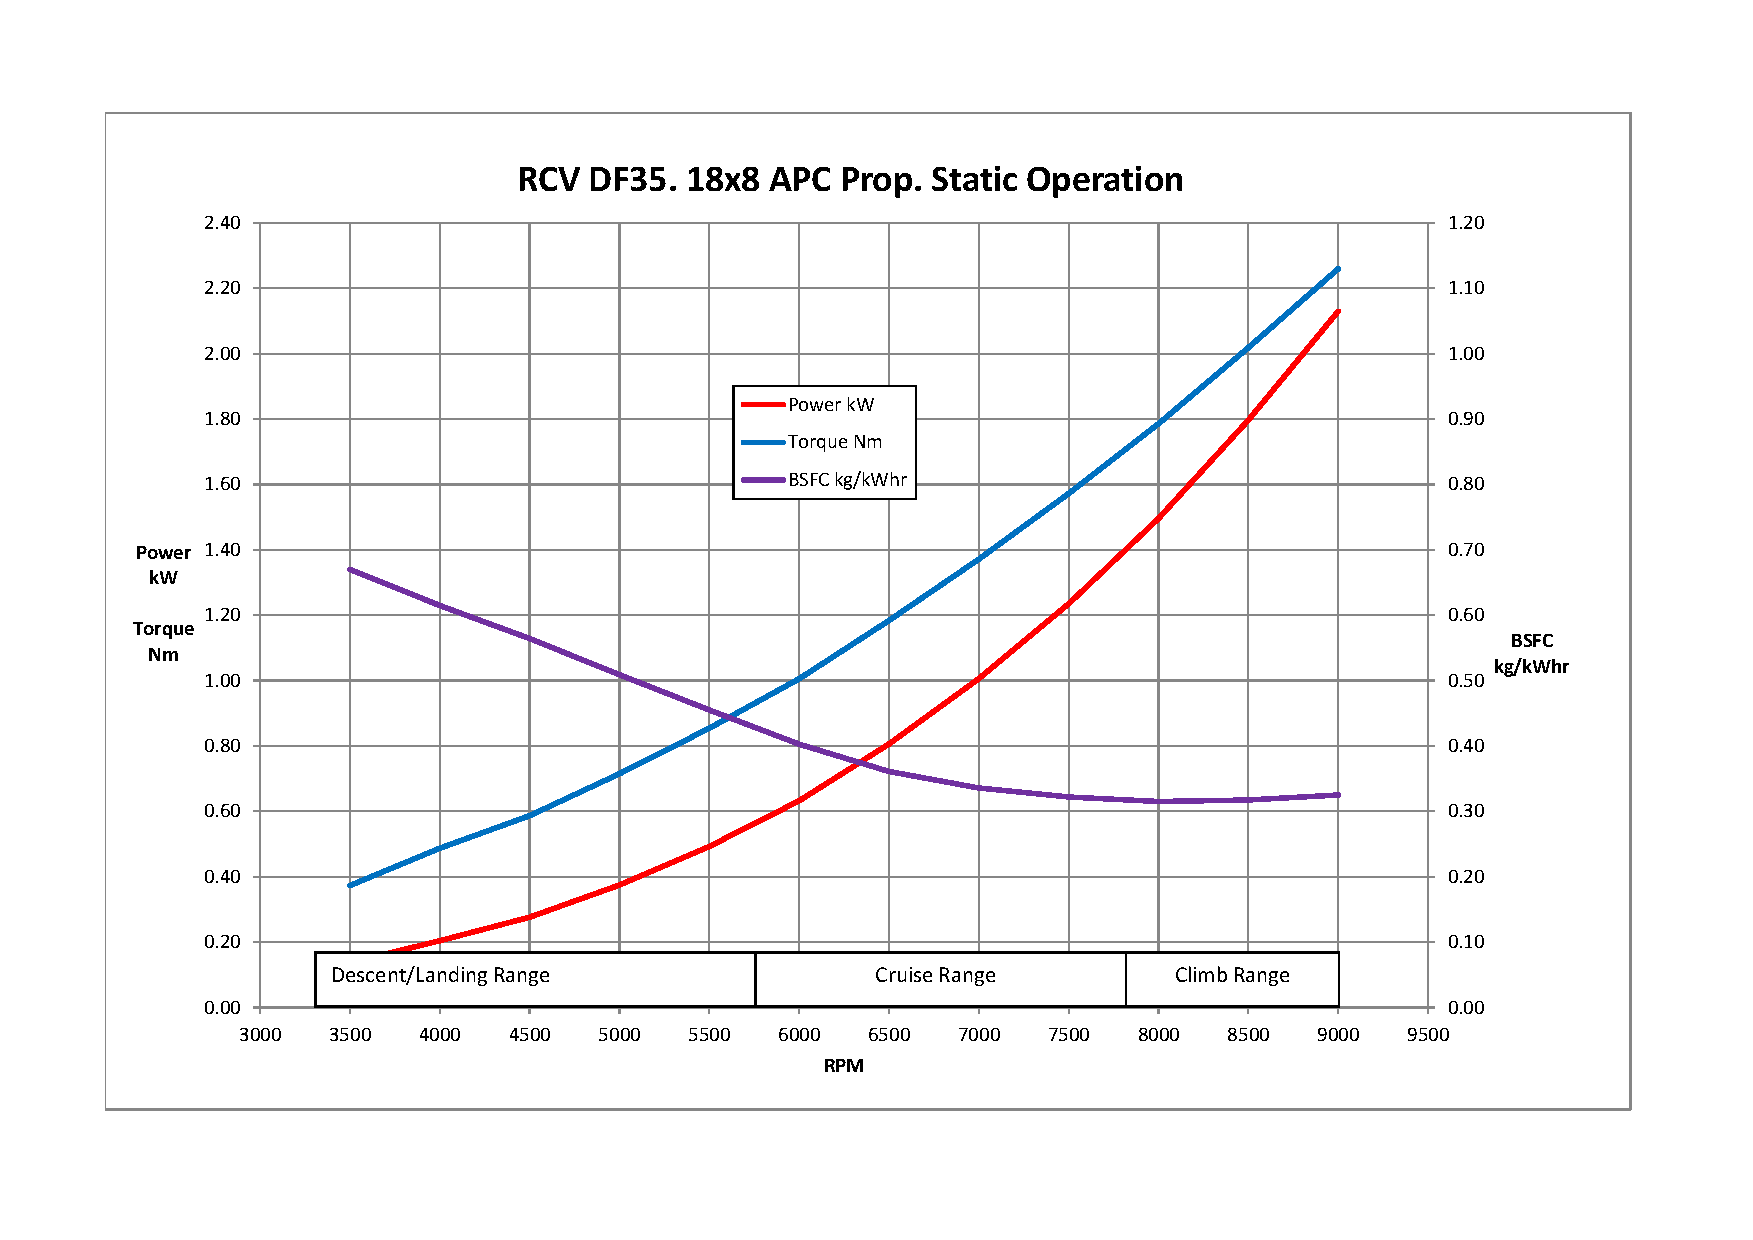
\includegraphics[scale = .4]{engineperf}
\caption{Engine Performance}
\end{center}
\end{figure}


\section*{Trade Studies}

\begin{figure}[h!]
\begin{center}
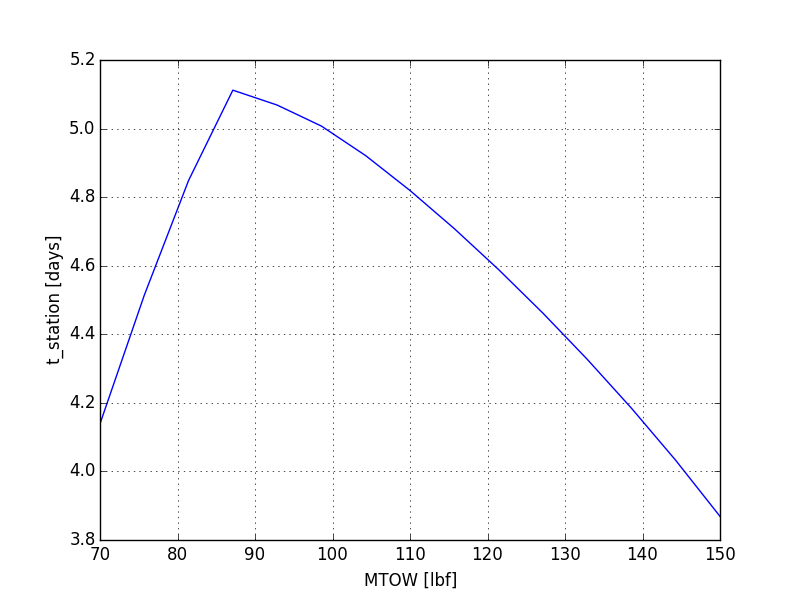
\includegraphics[scale = .6]{tvsMTOW}
\caption{Time on station vs MTOW.  This carries all the same assumptions.}
\end{center}
\end{figure}

\begin{figure}[h!]
\begin{center}
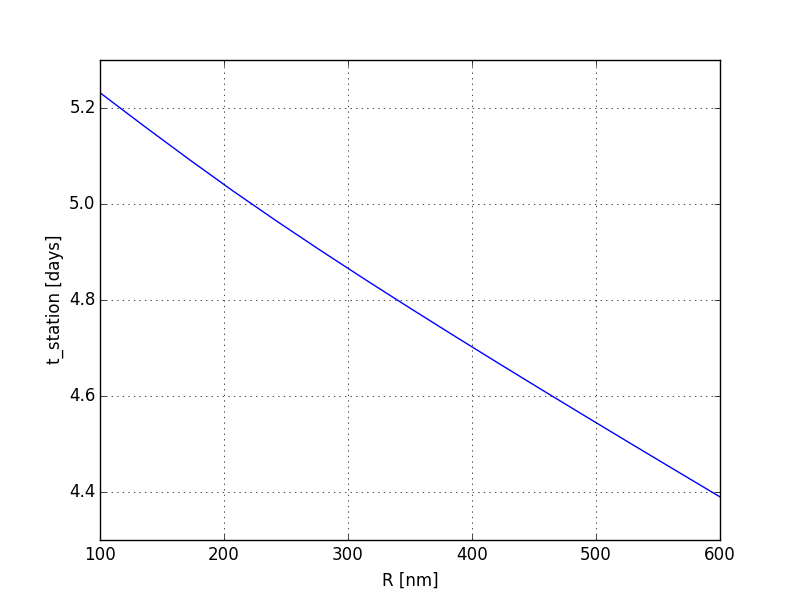
\includegraphics[scale = .6]{tvsR}
\caption{Time on station vs R. Assumes fixed weight of $MTOW = 87$ [lbf].}
\end{center}
\end{figure}

\begin{figure}[h!]
\begin{center}
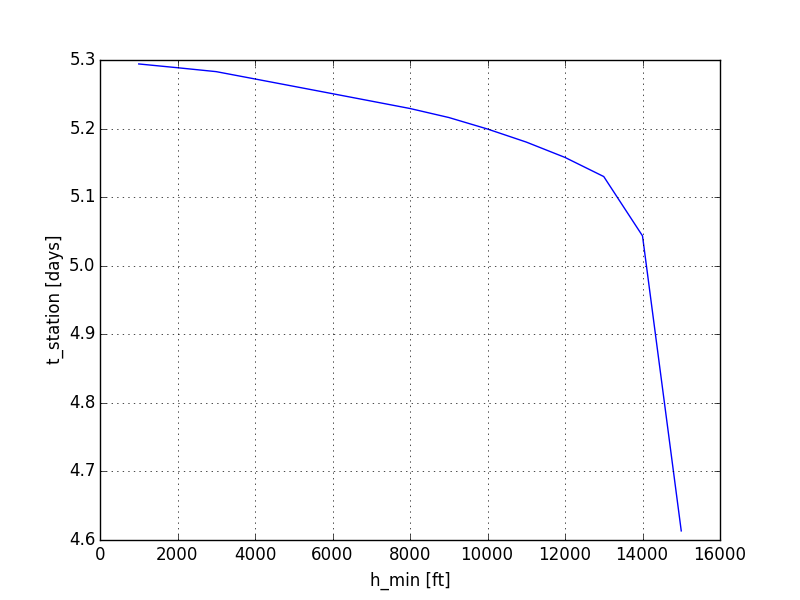
\includegraphics[scale = .6]{tvsh_min}
\caption{Time on station vs cruise altitude. Assumes fixed weight of $MTOW = 87$ [lbf].}
\end{center}
\end{figure}

\begin{figure}[h!]
\begin{center}
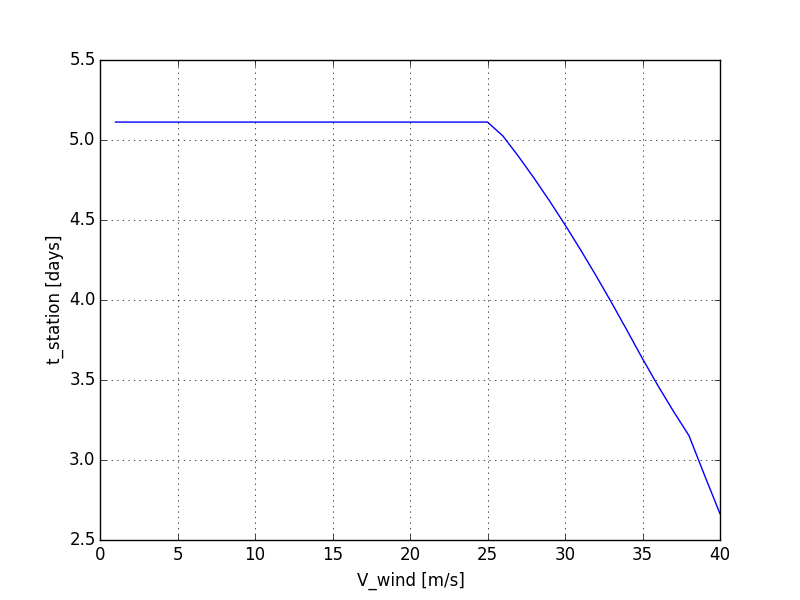
\includegraphics[scale = .6]{tvsV_wind}
\caption{Time on station vs wind velocity.  Assumes fixed weight of $MTOW = 87$ [lbf].}
\end{center}
\end{figure}

\begin{figure}[h!]
\begin{center}
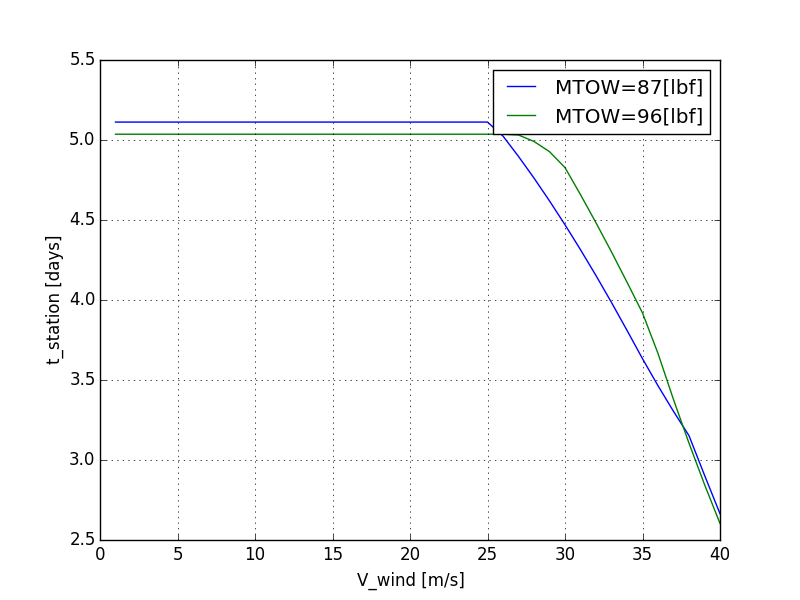
\includegraphics[scale = .6]{tvsV_wind96}
\caption{Time on station vs wind velocity. } 
\end{center}
\end{figure}

\end{document}
